\documentclass[a4paper,12pt,twoside]{report}

\usepackage{acronym}
\usepackage{url}
\usepackage{cite}
\usepackage{listings}
\usepackage[pdftex]{graphicx}
\usepackage[hang,small,bf]{caption}
\usepackage{styles/tum}
\usepackage{styles/usecases}
\usepackage{setspace}
\usepackage[german,english]{babel}
\usepackage{float}
\usepackage{floatflt}
\usepackage{fancyhdr}
\usepackage{color}
\usepackage{booktabs}
\usepackage[pdftex,bookmarks=true,plainpages=false,pdfpagelabels=true]{hyperref}
\usepackage{mdwlist}
\usepackage{enumerate}
\usepackage{paralist}
\usepackage{array}
\usepackage{longtable}
\usepackage{listings}
\usepackage[utf8]{inputenc}
\usepackage[capitalize, noabbrev]{cleveref}

% Path for graphics
\graphicspath{{figures/}}

\begin{document}
\setlength{\evensidemargin}{22pt}
\setlength{\oddsidemargin}{22pt}

\def\doctype{Master's Thesis}
\def\faculty{Informatik}
\def\title{Using Synthetic Data for Classification of Small Parts}		%TODO add title in German
\def\titleGer{Synthetische Daten für die Klassifizierung von Kleinteilen verwenden}	%TODO add title in German
\def\supervisor{Prof. Bernd Brügge, Ph.D.}
\def\advisor{Sajjad Taheri, M.Sc.}
\def\author{Amr Abdelraouf}
\def\date{15.10.2018}		%TODO add submission / handover date


\hypersetup{pdfborder={0 0 0},
                        pdfauthor={Amr Abdelraouf},
                        pdftitle={Using Synthetic Data for Classification of Small Parts},
                        }

\lstset{showspaces=false, numbers=left, frame=single, basicstyle=\small}

\pagenumbering{alph}

\thispagestyle{empty}

\vspace{4cm}
\begin{center}
\oTUM{4cm}\\ 
\vspace{5mm}     
\huge FAKULT{\"A}T F{\"U}R INFORMATIK\\ 
\vspace{0.5cm}
\large DER TECHNISCHEN UNIVERSIT{\"A}T M{\"U}NCHEN\\
\vspace{1mm}
\end{center}

\vspace{13mm}

\begin{center}
{\Large \doctype\ in \faculty}
\vspace{20mm}

\begin{spacing}{1.5}
{\huge\bf \title}\\%[3ex]
\end{spacing}

\vspace{15mm}
{\LARGE \author}

\vspace{10mm}

\begin{figure}[h!]
\centering
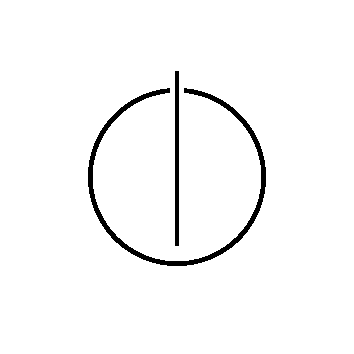
\includegraphics[width=4cm]{InformaticsLogo}
\end{figure}

\end{center}

\thispagestyle{empty}

\vspace{8mm}
\begin{center}
\oTUM{4cm}

\vspace{5mm}     
\huge FAKULT{\"A}T F{\"U}R INFORMATIK\\ 
\vspace{0.5cm}
\large DER TECHNISCHEN UNIVERSIT{\"A}T M{\"U}NCHEN\\
\end{center}

\vspace{5mm}

\begin{center}
{\Large \doctype\ in \faculty}
\vspace{8mm}

\begin{spacing}{1.3}
{\LARGE \title}\\
\vspace{8mm}

{\LARGE \titleGer}\\
\vspace{8mm}
\end{spacing}

\begin{tabular}{ll}
\Large Author:     & \Large \author     \\[2mm]
\Large Supervisor: & \Large \supervisor \\[2mm]				
\Large Advisor:	   & \Large \advisor    \\[2mm]
\Large Date:       & \Large \date
\end{tabular}

\vspace{1mm}

\begin{figure}[hb!]
\centering
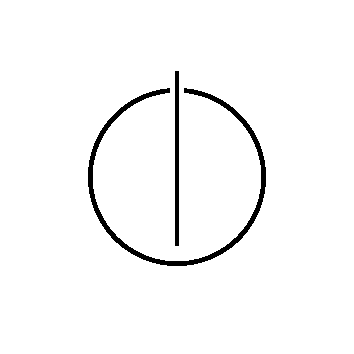
\includegraphics[width=4cm]{InformaticsLogo}
\end{figure}

\end{center}
\newpage
\thispagestyle{empty}
\mbox{}
\clearpage
\thispagestyle{empty}
\vspace*{0.8\textheight}
\noindent
I assure the single handed composition of this master thesis only supported by declared resources,

\vspace{15mm}
\noindent
Munich, \date \hspace{\stretch{1}} \author
\newpage



\newpage
\thispagestyle{empty}
\mbox{}

\chapter*{Acknowledgements}


\pagenumbering{roman}

\selectlanguage{english}
\begin{abstract}

Recent advances in Convolutional Neural Networks (CNN) have been able to conquer Computer Vision tasks and even surpass human performance. CNN algorithms are characteristically data-hungry, and obtaining domain-specific labeled data is often a cumbersome manual resource-heavy task. In this text we explore the use of synthetic data to train a CNN to perform image classification of different fasteners.

\textit{Note:}

\textit{\textbf{1. paragraph:} What is the motivation of your thesis? Why is it interesting from a scientific point of view? Which main problem do you like to solve?}

The motivation for my thesis stems from CNN algorithms' hunger for labeled images in order to train for classification tasks and produce performant results. Obtaining a large corpus of labeled images is a difficult task, especially when we wish to train a network to classify a domain-specific dataset.

\textit{\textbf{2. paragraph:} What is the purpose of the document? What is the main content, the main contribution?}
In this document we explore the use of synthetic images to augment the training data for a given CNN. We explore the power of synthetic data to produce acceptable results while using as little real data as possible. The intuition comes from the ease of rendering a large synthetic dataset on demand.

\textit{\textbf{3. paragraph:} What is your methodology? How do you proceed?}
We explore the ratio of synthetic to real images that can be used for training a CNN and obtain good results.

\end{abstract}

\clearpage

\selectlanguage{english}

\tableofcontents
\clearpage

\pagenumbering{arabic}

\fancyhead{}
\pagestyle{fancy}
\fancyhead[LE]{\slshape \leftmark}
\fancyhead[RO]{\slshape \rightmark}
\headheight=15pt










%------- CHAPTER 1 -------

\chapter{Introduction}

Engine overhaul is the process of removing, disassembling, inspecting, repairing, cleaning, reassembling and testing a used engine. Overhauling involves the intricate process of dismantling an engine into small mechanical parts—ie. screws, fasteners, nuts and bolts. Those small mechanical parts are later reassembled back into a functioning engine.

Thousends of different small mechanical parts can be used to structure an engine. To facilitate the process of reassembling the engine, each small mechanical part has to be labeled with its position and function after it has been dismantled.

Traditionally, the task of labeling small mechanical parts is executed manually by a human task force. This approach presents a number of problems. Firstly, it is a labour-intensive task that depletes human resources. The manual approach requires a large number of man-hours to be invested, which means that it is both time consuming and expensive. Furthermore, labeling small mechanical parts is a sensitive process within the context of reassembling an engine. Humans are prone to error, which means that the manual approach would require further investment to ensure the accuracy of the labels that are assigned to the small mechanical parts.

In this thesis, we present an approach to automatically classify small mechanical parts using a camera. Our approach involves minimal human interaction, and thus slashes the amount of man power required to label small mechanical parts. Moreover our automatic approach provides a quantifiable measurment for accuracy which can be used to assess and imporve the system, and ultimately reduce the effort required to avoid misclassification errors.

Deep convolutional neural networks (CNNs) have become the state-of-the-art approach to classical computer vision and image processing tasks such as image classification, object detection and many others \cite{krizhevsky2012imagenet} \cite{szegedy2015going}. In this thesis we attempt to leverage the power of CNNs to automatically classify small mechanical parts during an engine overhauling process.

\section{Problem}

Deep convolutional neural networks are charactaristically data-hungry algorithms. The performance of a CNN algorithm is proportional the amount of data that is fed in as input. In our problem's case, we need to use a large number of images of each small mechanical part as input to the CNN algorithm. Creating a large number of images for our particular set of small mechanical parts is a time consuming and labour-intensive task. It presents the same problems as the traditional approach of manually labeling small mechanical parts.

In this thesis we propose an experiment to evaluate the use of synthetic images as input to CNN algorithms. Instead of using pictures of the small mechanical parts, we obtain their respective 3D models and use them to generate synthetic images of the real objects.

\section{Motivation}

Most of the cutting edge research in convolutional neural networks has been done using a large number of input data \cite{krizhevsky2012imagenet} \cite{simonyan2014very} \cite{szegedy2015going} \cite{he2016deep}, exploiting large corpora of labeled images \cite{deng2009imagenet}. CNN algorithms are much less effective at classifying images if a large amount of input data is absent.

Using synthetic images to classify small mechanical objects exploits the power of convolutional neural network while overcoming its main drawback: the need for a large number of input images. This approach is extendible to image classification problems in other domains. Synthtic images provide a fast and easy source of input to CNN algorithms without the impedence of having to create a large dataset.

Furthermore, the process of generating synthetic images gives full control of the surrounding environment to the creator of the synthetic scene. The synthetic scene can easily be adjusted to capture specific features of the small mechanical parts.

\section{Objectives}

The main objective of this thesis is to assess the use of synthetic data as input for CNN algorithms to perform image classification. We explore the use of a fully synthetic dataset and also a mixed dataset of both real and synthetic images with varying ratios.

\section{Outline}

The Background chapter provides an explanation of the technology used to fulfill the objective of this thesis. The Related Work section transcribes the literature that was reviewed in preparation for this thesis.

The Analysis chapter breaks down and presents the requirements of the software system that was used to execute our experiments. While the System Design chapter provides an extensive explanation of the system implementation details.

The Evaluation chapter contains our expirement design and results. Lastly, the Summary chapter contains a recap of our work, the conclusions we have reached and the potential future work that can be based on our thesis.










%------- CHAPTER 2 -------

\chapter{Background}

\textit{Note: Describe each proven technology / concept shortly that is important to understand your thesis. Point out why it is interesting for your thesis. Make sure to incorporate references to important literature here.}

\section{Supervised Machine Learning}
\subsection{Overview}
\subsection{Image Classification}

\section{Deep Neural Networks}

\section{Convolutional Neural Networks (CNNs)}
\subsection{CNN Building Blocks}
\subsection{CNN Architectures}
\subsubsection{VGG16}
\subsubsection{VGG19}
\subsubsection{Resnet}
\subsubsection{Inception}

\section{Small Mechanical Part Classification}










%------- CHAPTER 3 -------

\chapter{Related Work}

\textit{Note: Describe related work regarding your topic and emphasize your (scientific) contribution in \textbf{contrast} to existing approaches / concepts / workflows. Related work is usually current research by others and you defend yourself against the statement: ``Why is your thesis relevant? The problem was already solved by XYZ.'' If you have multiple related works, use subsections to separate them.}

\section{CNN based Image Classification}
\section{Image Classification using Synthetic Images}










%------- CHAPTER 4 -------

\chapter{Analysis}

%\textit{Note: This chapter follows the Requirements Analysis Document Template in \cite{bruegge2004object}. 
%\textbf{Important:} Make sure that the whole chapter is independent of the chosen technology and development platform. The idea is %that you illustrate concepts, taxonomies and relationships of the application domain independent of the solution domain!
%Cite \cite{bruegge2004object} several times in this chapter.}

\section{Overview}

Our goal is to develop a system that classifies images of different small mechanical parts (SMPs), and to do so as accurately as possible. To realize this goal, we decide to leverage state-of-the-art advancements in Convolutional Neural Network algorithms in the field of computer vision, and more specifically, the sub-field of image classification.

We aim to build a system that scales up well, ie. we would like the classification system to easily adapt new small mechanical parts. Moreover we would like to build a system that can scale up to around 10,000 classes.

CNN algorithms are characteristically data-hungry. The classification accuracy of a CNN algorithm is proportional to the amount of images that are fed in as input. Given the large number of classes, the task of collecting images of each small mechanical part becomes time-consuming and labour-intensive. To combat this problem, we decide to augment the training data of our algorithms with \textit{synthetic images}: 2-dimentional renditions of 3-dimensional computerized graphical models of the small mechanical parts. We hypothesize that our synthetically augmented training set will yield a higher accuracy, whilst minimizing the manual effort needed to take real images of the small mechanical parts.

\section{Requirements}

\subsection{Functional Requirements}

Functional requirements (FRs) describe the interactions between the system and the its environment independent of its implementation. \cite{bruegge2004object}.

The system's main function is to classify images of different small mechanical parts. Furthermore, the system needs to be dynamic and scalable to accomodate new small mechanical parts. To ensure that the system is able to classify images accurately, while leveraging synthetic input images, we introduce the folloing Functional Requirements.

\begin{itemize}
  \item [FR1] \textbf{Generate Synthetic Images}: Given a 3D model of a small mechanical part, the system should generate a set of synthetic images of said model. The system should apply a set of random transformations to the 3D model before rendering the 2D synthetic image to ensure that the generated dataset captures the SMP from as many angles in as many positions as possible.

  \item [FR2] \textbf{Add New Class to Image Classifier}: The system should accomodate the addition of a new SMP to the classifier. This extends to the ability of the system to accomodate for new input training data, and the ability to label a new output class

  \item [FR3] \textbf{Adjust input data split}: The system should allow for changes in the training, validation and testing input data which is assigned as input to the image classifier. This includes changing the number of images in each set and manipulating the ratio of synthetic to real images in the training split.

  \item [FR4] \textbf{Retrain Image Classifier}: The system should be dynamic enough to retrain the image classifier. This step is usually taken after the augmenting or adjustment of the input data split.

  \item [FR5] \textbf{Fine-Tune Image Classifier}: The underlying CNN algorithm should be subject to fine-tuning in order to maximize the accuracy of the system.
\end{itemize}

\subsection{Nonfunctional Requirements}

Nonfunctional Requirements (NFRs) are key system requirements that apply to the system as a whole. To maintain the system's general requirements we define the following nonfunctional requirements.

\begin{itemize}
  \item [NFR1] \textbf{Performance}: A performence requirement is the measure of a quantifiable attribute of our system. In our case we would like to track our system's \textbf{classification accuracy}.\\
  We first specify our system's accuracy for a single class to be the percentage of the given class's testing image split that the image classifier correctly predicts. We consequently define our system's classification accuracy to be the image classifier's average prediction accuracy over each class.

  \item [NFR2] \textbf{Adaptability}: Adaptability is the ability to change the system to deal with additional application domain concepts \cite{bruegge2004object}. Our system needs to be dynamic enough to accomodate for new small mechanical parts that can be later added even after the system has been deployed.
\end{itemize}

\section{System Models}

\subsection{Use Case Model}

Use case models represent the relationship between the user group of a system and the general functions that they can execute. A use case model can reduce the complexity of a system and increase its understandability.

The use case model of our system can be found as figure [\ref{fig:UCM}]. The main protagonist of our system is the mechanical engineer who is tasked with training the system to classify a set of small mechanical parts.

\begin{figure}[h]
\centering
  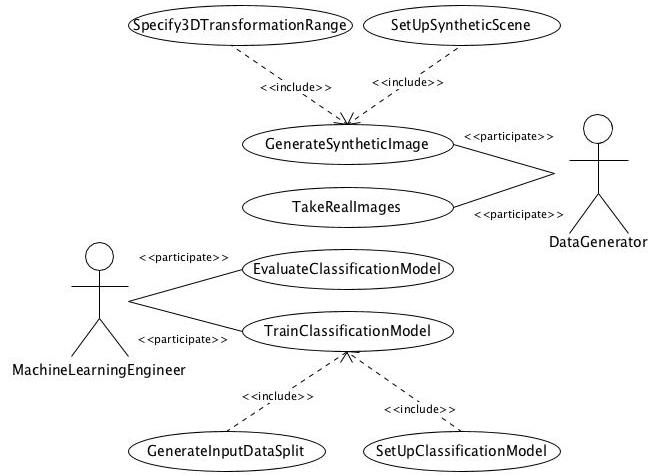
\includegraphics[width=\textwidth]{UCM}
\caption{Use Case Model}
\label{fig:UCM}
\end{figure}

The use case model can be divided into 3 main functions; namely generating synthetic images, obtaining real images, and training an image classifier.

\subsubsection{Generating Synthetic Images}

Generating synthetic images the cornerstone for a synthetically augmented dataset. There's a lot of work that goes into generating the 3D synthetic scene and the corresponding renditions. To increase the understandability of our model, we have separated the the use case that revolve around modeling the SMP 3D model itself as \textit{Specify3DModelTransformations}, and the use case that deals with the synthetic scene environment as \textit{SetUpSyntheticScene}.

\begin{usecase}
  \addtitle{Use Case}{Specify3DModelTransformations}

  \addfield{Participating Actors}{DataCollector}

  \addscenario{Flow of Events}{
    \item In the modeling software, the DataCollector chooses the transformations that are applicable to the small mechanical part's 3D model.
    \item For each transformation, the DataCollector sets the range of each tranformation attribute that will be later used to generate a random position for the synthetic image of the SMP.
  }

  \addfield{Entry Condition}{DataCollector has modeling software open.}

  \addfield{Exit Condition}{All the desired transformations and their corresponding attributes have been specified.}

  \additemizedfield{Quality Requirements}{
    \item In the effort to achieve the Performance Non-Functional requirement, synthetic images have to look as photo realistic as possible. The 3D transformations should strive to output the range of positions that the respective SMP can be placed in.
  }
\end{usecase}

\clearpage
\begin{usecase}
  \addtitle{Use Case}{SetUpSyntheticScene}

  \addfield{Participating Actors}{DataCollector}

  \addscenario{Flow of Events}{
    \item In the modeling software, the DataCollector places the 3D model of the SMP on a horizontal plane as if lying on a table.
    \item The DataCollector sets the background of the horizontal plane to mimic the background of the real images in the dataset.
    \item The DataCollector sets the lighting condition of the scene to reflect the lighting condition of the environment where the real SMP images are taken.
  }

  \addfield{Entry Condition}{DataCollector has modeling software open.}

  \addfield{Exit Condition}{In the modeling software, the 3D model of the SMP should be lying on a horizontal plane with a background and lighting condition that reflect the environment of the real SMP images.}

  \additemizedfield{Quality Requirements}{
    \item The synthetic scene should look as photorealistic as possible. This helps the Image Classifier achieve a higher classification accuracy using the synthetic images.
  }
\end{usecase}

\clearpage
\begin{usecase}
  \addtitle{Use Case}{GenerateSyntheticImages}

  \addfield{Participating Actors}{DataCollector}

  \addscenario{Flow of Events}{
    \item The DataCollector specifies the desired number of output synthetic images.
    \item The modeling software generates the desired number of output synthetic images. Each image is a rendition of the scene after the transformations have been applied to the 3D model.
  }

  \addfield{Entry Condition}{DataCollector has modeling software open.}

  \addfield{Exit Condition}{The DataCollector obtains a set of synthetic images for the specified SMP that can be later used to train the Image Classifier.}
\end{usecase}

\clearpage
\subsubsection{Obtaining Real Images}

\begin{usecase}
  \addtitle{Use Case}{TakeRealImages}

  \addfield{Participating Actors}{DataCollector}

  \addscenario{Flow of Events}{
    \item The DataCollector places the camera over a plane.
    \item The DataCollector sets the SMP over the plane in a random position, such that the full SMP body is within the viewfield of the camera.
    \item The DataCollector takes a picture of the SMP.
    \item The DataCollector repeats steps 2 and 3 until the desired number of real images of the SMP is reached.
    \item The DataCollector resizes the images to correspond to the input image size of the Image Classifier. 
  }

  \addfield{Entry Condition}{}

  \addfield{Exit Condition}{The DataCollector obtains a set of real images for the specified SMP that can be later used to train the Image Classifier.}

  \additemizedfield{Quality Requirements}{
    \item The lighting of the environment should eliminate shadows and light reflections on the SMP surface.
  }
\end{usecase}

\clearpage
\subsubsection{Training the Image Classifier}

Training the image classifier requires some underlying work. We have chosen to model this use case as one that includes setting up the input data and configuring the image classifier (modeled as \textit{SetInputDataSplit} and \textit{SetUpImageClassifier} respectively).

\begin{usecase}
  \addtitle{Use Case}{TrainImageClassifier}

  \addfield{Participating Actors}{MachineLearningEngineer}

  \addscenario{Flow of Events}{
    \item The MachineLearningEngineer configures the dataset structure: number of images for training, validation and testing, as well as the ratio of real to synthetic images in the training split.
    \item The MachineLearningEngineer chooses a convolutional neural network architecture for the Image Classifier.
    \item The MachineLearningEngineer fine-tunes the CNN by manipulating its hyperparameters.
  }

  \addfield{Entry Condition}{For each SMP set to be classified by the Image Classifier, the corresponding real and synthetic images should be generated and ready for use.}

  \addfield{Exit Condition}{The Image Classifier outputs the maximum possible accuracy given the input dataset.}
\end{usecase}

\clearpage
\subsection{Analysis Object Model}

The analysis object model is a visual dictionary of the main concepts visible to the user \cite{bruegge2004object}. The analysis object model depicts a system's entites, their corresponding attributes and functions, and illustrates the relationship between said entitie. Figure [\ref{fig:AOM}] represents the analysis object model of our system.

\begin{figure}[h]
\centering
  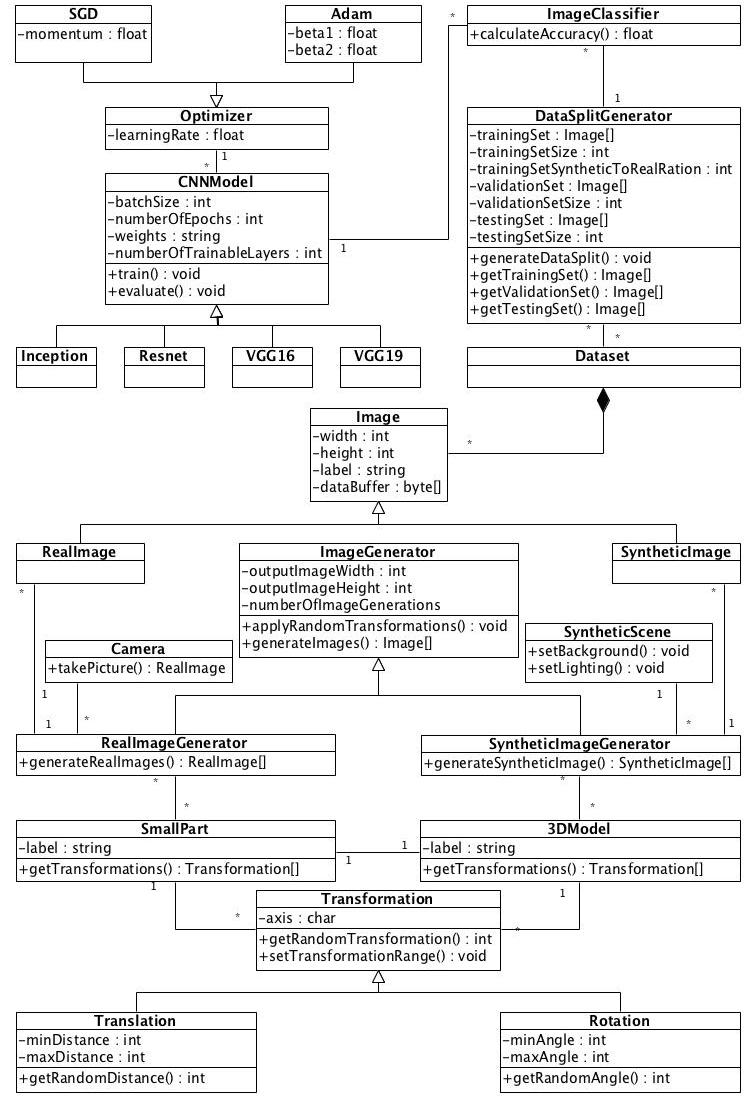
\includegraphics[width=\textwidth]{AOM}
\caption{Analysis Object Model}
\label{fig:AOM}
\end{figure}

\subsubsection{SmallMechanicalPart}
A small mechanical part is the main subject of our system. It is an object that our system aims to classify. Each SMP has a unique identifying label string.

\subsubsection{3DModel}
A 3DModel of a small mechanical part is the graphical model which helps our system create synthetic images. Each SMP has a corresponding 3DModel. Each 3DModel has the same label as its SMP counterpart.

\subsubsection{Transformation}
Each SMP and 3DModel have a list of applicable transformations. A transformation is executed on an axis (x, y or z), and can either be a Translation or a Rotation.
At image generation time, each transformation outputs a random value between its defined maximum and minimum. We define a range to limit an object's transformation. For instance, we don't want to translate an SMP so far as to remove it from the camera's viewfield.

\subsubsection{ImageGenerator}
ImageGenerator is the class that does the heavy lifting when it comes to creating images. It applies the random transformations on the target object and generates an image with a specified width and height.
ImageGenerator is an abstraction of 2 classes. SyntheticImageGenerator is responsible for applying the transformations on 3DModels, and using SyntheticScene to generate SyntheticImages, while RealImageGenerator uses a camera to take pictures of SmallMechanicalParts and output their corresponding RealImages.

\subsubsection{Image}
Image is a generalization of RealImage and SyntheticImage. Image stores information like width, height and label of the image. Moreover it contains a dataBuffer which contains the actual image pixel values.

\subsubsection{Dataset}
Dataset is a composition of Images. It is the image repository which is used by the ImageClassifier for training and evaluation.

\subsubsection{DataSplitGenerator}
DataSplitGenerator splits the Dataset into a training set, validation set and testing set. This split prepares the data for consumption by the ImageClassifier.

\subsubsection{CNNModel}
CNNModel is the convolutional neural network algorithm that is trained for image classification. CNNModel is an abstraction of 4 different CNN architectures, namely Inception, Resnet, VGG16 and VGG19. Furthermore, CNNModel defines the weights that are used to initialize the CNN to leverage the power of transfer learning. CNNModel also sets the number of trainable layers in a network to potentially preserve the initial weights and speed up training.

\subsubsection{Optimizer}
Each CNNModel has an Optimizer. An Optimizer is the function aims to close the gap between the model's predictions of the validation set labels and their corresponding ground truth. The Optimizer operates in the CNNModel's training phase. Optimizer is an abstraction of 2 different optimizers that we use in our system. Specifically SGD (Stochastic Gradient Descent), and Adam.

\subsubsection{ImageClassifier}
ImageClassifier orchestrates the feeding of data into the CNNModel for training. Moreover, it uses the testing set to calculate the accuracy of the trained model.


\subsection{Dynamic Model}

The dynamic model is focused on the behavior of the system. Sequence diagrams, activity diagrams and state machines are usually used to depict dynamic models \cite{bruegge2004object}. In this section we present 2 activity diagrams that depict the 2 main workflows of our system.

\subsubsection{Dataset Generation}

Figure [\ref{fig:AD1}] depicts the workflow of activities required to generate a dataset. The DataCollector selects a small mechanical part and its corresponding 3D model. The DataCollector then proceeds to generate the real and synthetic images. Finally the images are combined to form a dataset.

\begin{figure}[h]
\centering
  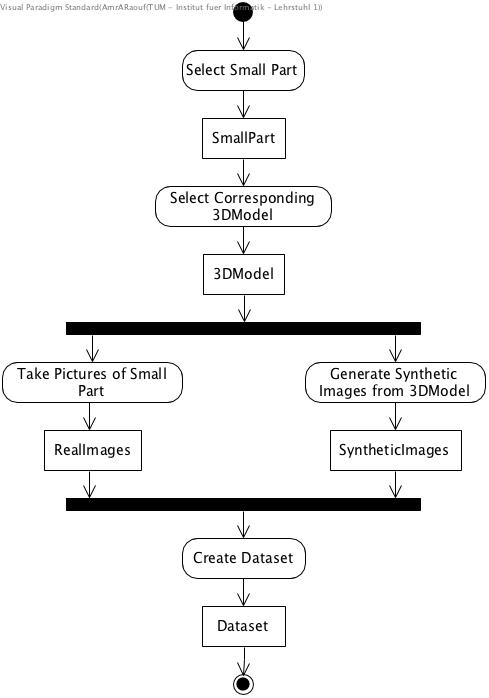
\includegraphics[width=\textwidth]{AD1}
\caption{Activity Diagram depicting the workflow required for Dataset generation}
\label{fig:AD1}
\end{figure}

\subsubsection{Training the Image Classifier}

Figure [\ref{fig:AD2}] describes the workflow of activities required to train the image classifier. The MachineLearningEngineer splits the data into training, validation and testing sets. The MachineLearningEngineer then creates a CNN model. Next the MachineLearningEngineer feeds the training data to the CNN model to obtained a trained CNN model. The MachineLearningEngineer then evaluates the trained CNN model accuracy using the testing set. If the accuracy of the trained CNN model is not sufficient, the CNN model is fine tuned and re-trained.

\begin{figure}[h]
\centering`
  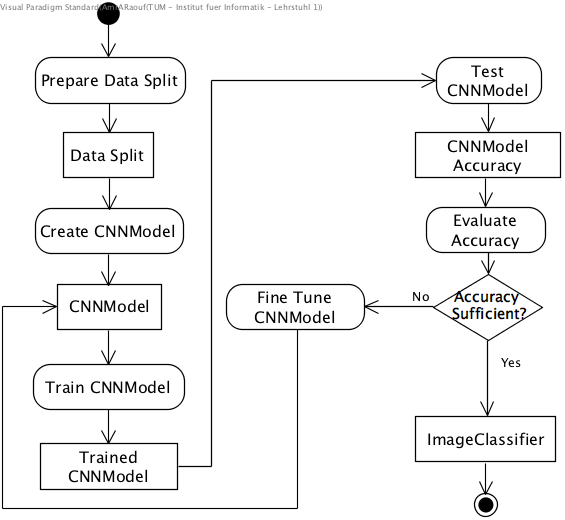
\includegraphics[width=\textwidth]{AD2}
\caption{Activity Diagram describing the workflow required to train the Image Classifier}
\label{fig:AD2}
\end{figure}









%------- CHAPTER 5 -------

\chapter{System design}

\section{Overview}

In the previous chapter, we have extracted the functional and non-functional requirements of our system. We then broke down our system into use cases in the Use Case Model [\ref{fig:UCM}]. Furthermore, we have described the entities of our system and the relationships between them using an Analysis Object Model [\ref{fig:AOM}].

In this chapter we map our analysis into the solution domain. We group the objects that we have identified in the Analysis Object Model [\ref{fig:AOM}] into subsystems. The implementation details of our subsystems and the dependencies between them are also discussed.

\section{Design Goals}

In the previous chapter we have defined our Non-functional requirements. In this chapter, we use those non-functional requirements to extract our design goals, and we use those design goals as a compass for our system design. Defining our design goals allows us make consistent design decisions accross our different subsystems. Table [\ref{tab:DG}] lists our non-functional requirements and their corresponding design goal. There are 5 types of possible design criteria from which the design goals can be selected: performance, dependability, cost, maintenance and end user criteria \cite{bruegge2004object}.

\begin{table}
  \centering
  \begin{tabular}{ | l | p{5cm} | l | }
    \hline
    \textbf{Requirement} & \textbf{Design Goal} & \textbf{Criteria} \\ \hline
    \textbf{Accuracy} & The system should be dynamic enough to accomodate the addition of new classes. & Performance \\ \hline
    \textbf{Adaptability} & The system should be able to classify different small mechanical parts with high accuracy. & Performance \\ \hline
  \end{tabular}
  \caption{Non-functional requirements and their corresponding design goals}
  \label{tab:DG}
\end{table}

\section{Subsystem Decomposition}

Figure [\ref{fig:SSD}] depicts the system's subsystem decomposition. Our system is divided into 3 subsytems: SyntheticImageServer, RealImageServer and ImageClassifier.

\subsection{SyntheticImageServer}
SyntheticImageServer is responsible for providing our system with synthetic images. It consists of 2 main components: SyntheticScene and SyntheticImageGenerator. The SyntheticScene generates an artificial environment and places a 3DModel inside said environment. The SyntheticImageGenerator renders 2D images of the 3D artificial scene.

\subsection{RealImageServer}
The RealImageServer is the SyntheticImageServer's counterpart. It is responsible for providing our system with real images. The RealImageGenerator uses the Camera to take real images of the small mechanical parts. Next, the RealImageGenerator performs some processing on the raw images to provide our system with real images that can be used out of the box.

\subsection{ImageClassifier}
ImageClassifier consumes both the real and syntheic images, and stores them in a Dataset. The images are then fed to the DataSplitGenerator, which is in turn responsible for splitting the data into a training set, a validation set and a testing set.

The CNNModel consumes the training set and the validation set to utilize them during the training phase. The testing set is then used to determine the accuracy of the trained CNNModel.

\begin{figure}[h]
\centering
  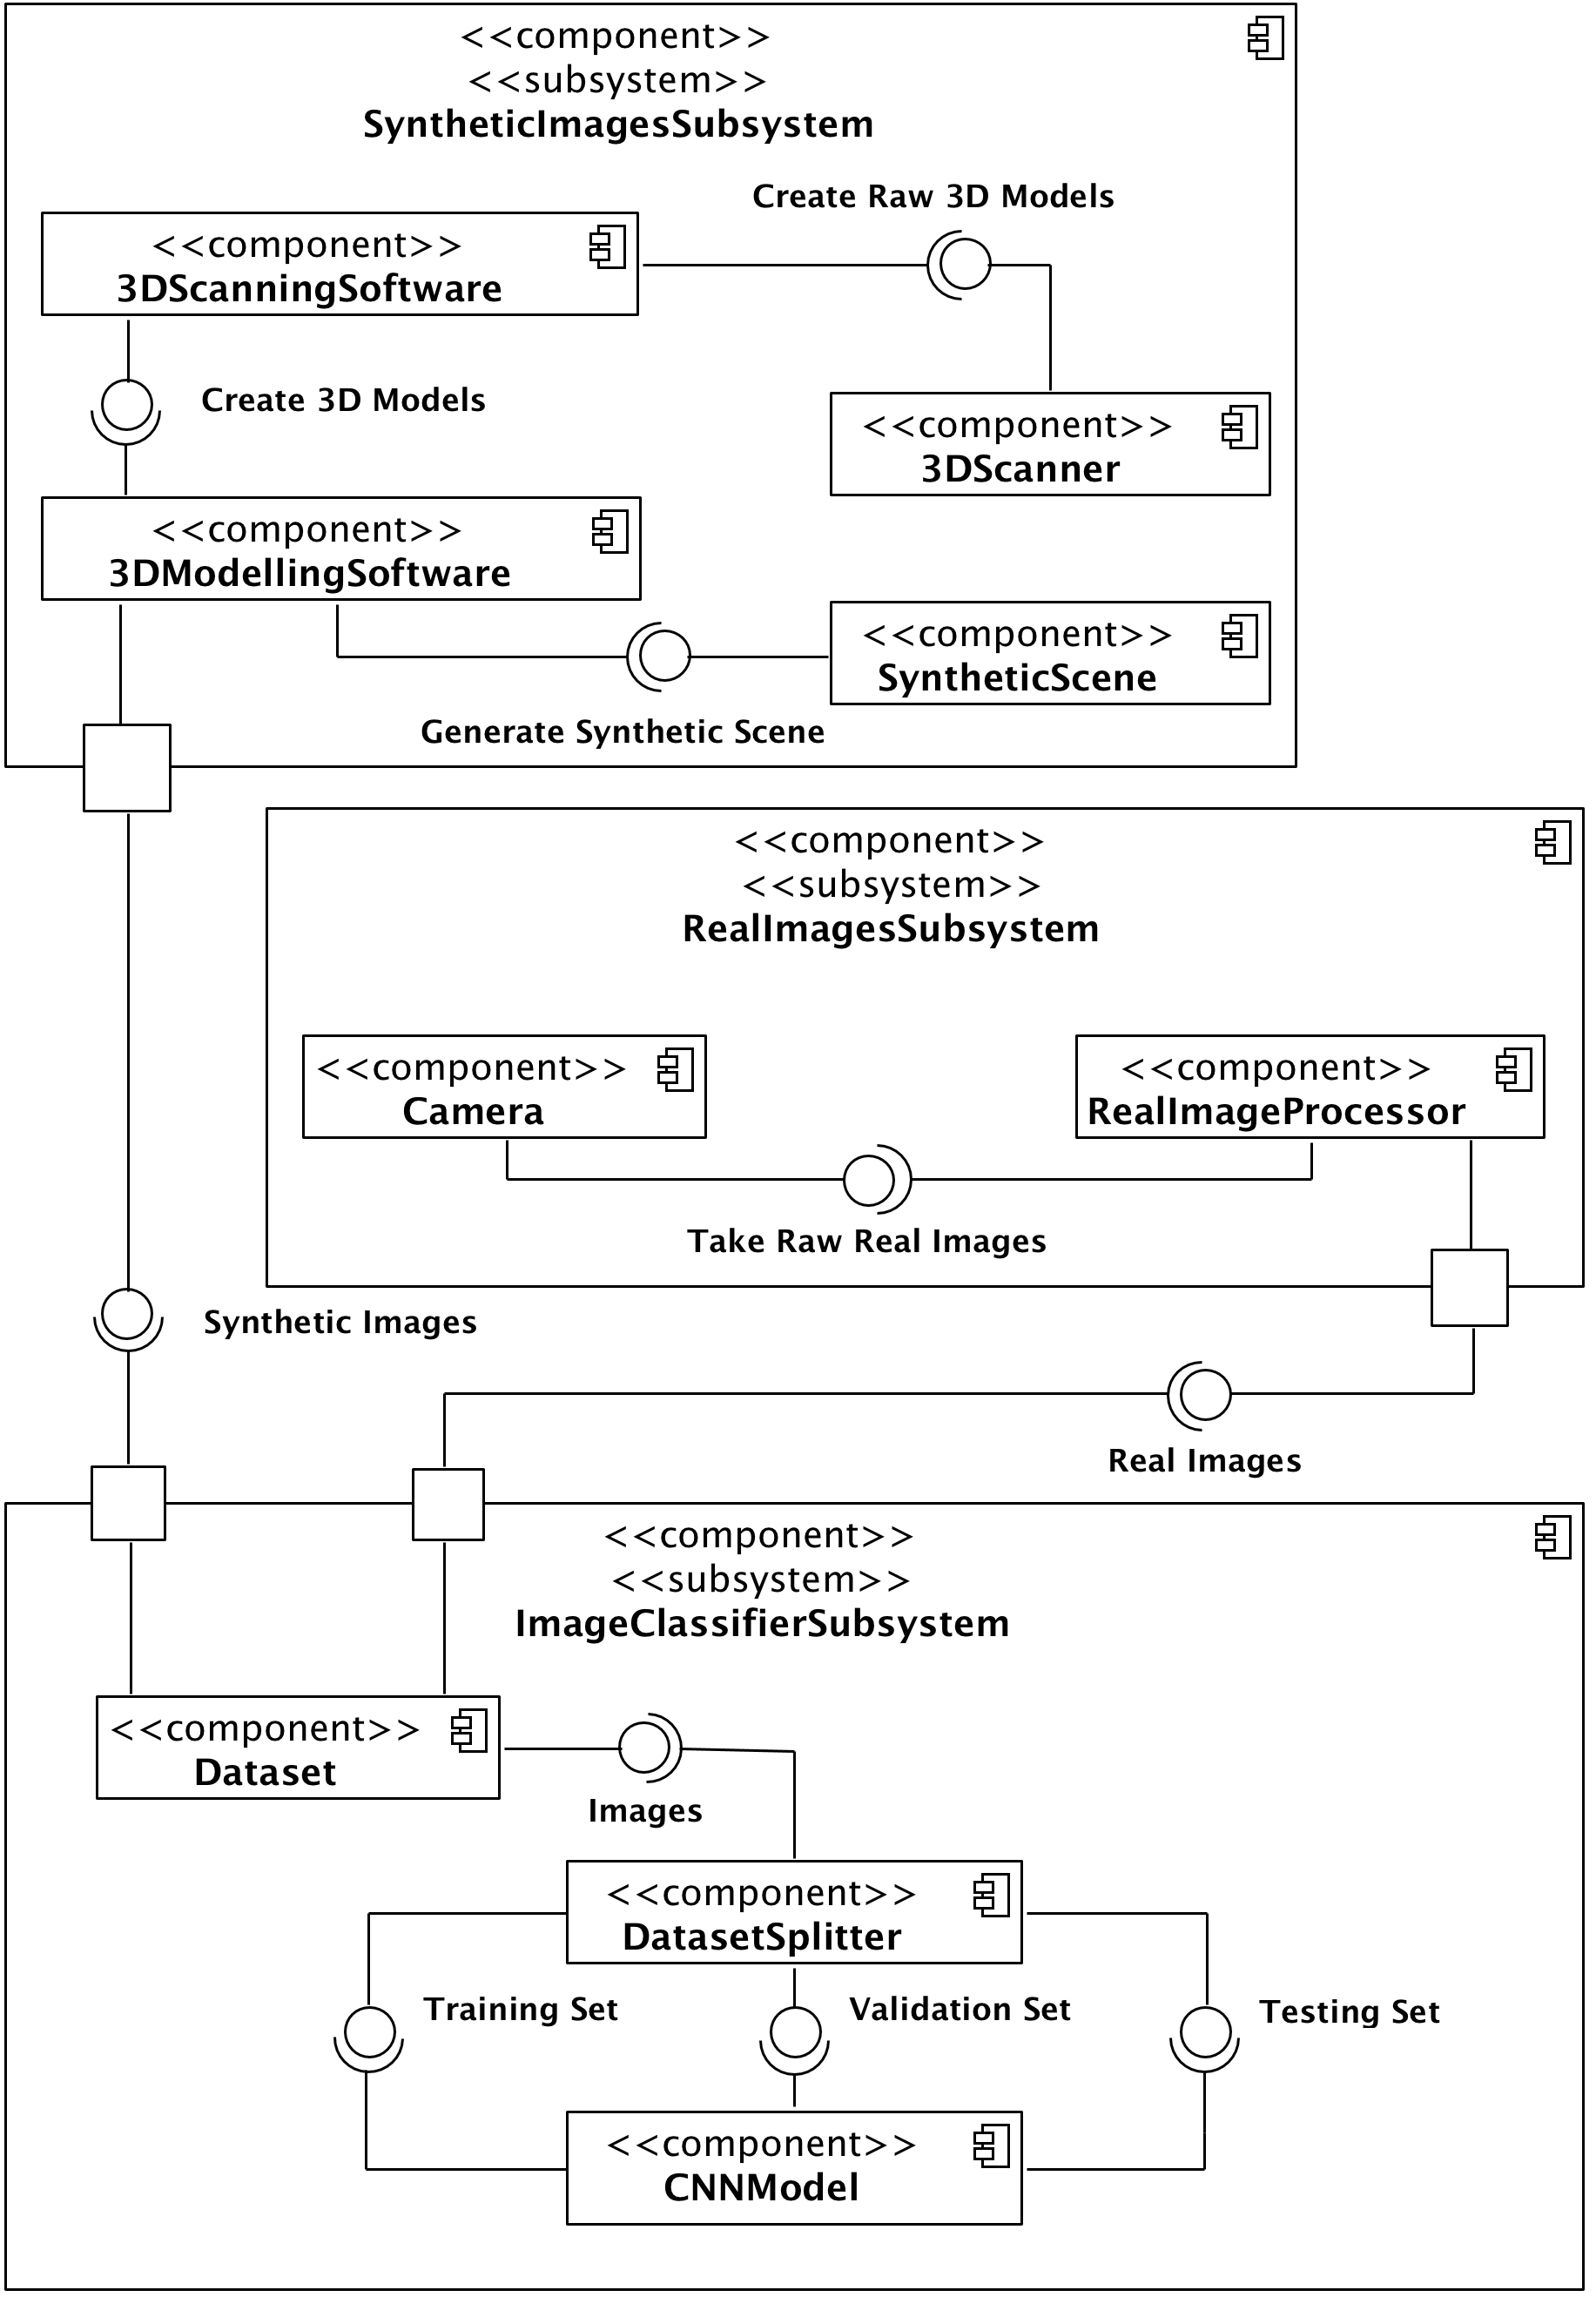
\includegraphics[width=\textwidth]{SSD}
\caption{Subsystem Decomposition}
\label{fig:SSD}
\end{figure}

\section{Hardware Software Mapping}
This section describes how the subsystems are mapped onto existing hardware and software components. Figure [\ref{fig:DD}] depicts the deployment diagram of our system. Our system contains 4 hardware devices: 2 Ubuntu machines, a Windows machine and a Camera.

\begin{figure}[h]
\centering
  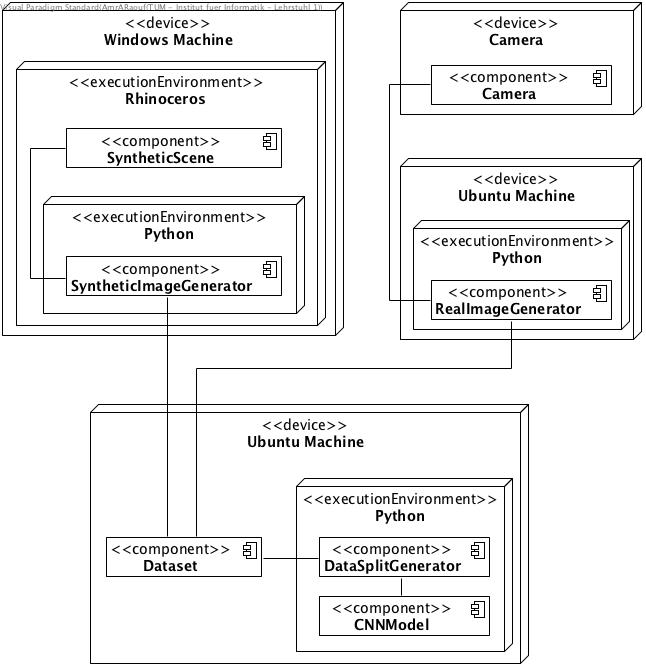
\includegraphics[width=\textwidth]{DD}
\caption{System Deployment Diagram}
\label{fig:DD}
\end{figure}

\subsection{Windows Machine}
The Windows machine is used to run the Rhinoceros 3D modeling software. We chose the windows version of Rhinoceros because it features that are not available on the Ubuntu or Mac versions. We use Rhinoceros to model the SyntheticScene. Moreover, Rhinoceros hosts a python interpreter, which we use to run the SyntheticImageGenerator.

\subsection{Camera}
The Camera is used to capture raw images of the small mechanical parts.

\subsection{Ubuntu Machine}
The RealImageGenerator uses the Camera to generate raw real images. The raw real images are then processed by the RealImageGenerator and become ready to be used out of the box.

\subsection{Ubuntu Machine}
The second Ubuntu machine is used to run the ImageClassifier. The Dataset is stored in the Ubuntu machine's file system. We use the system's Python environment to run the DataSplitGenerator and the CNNModel. This Ubuntu Machine is equipped with a Graphics processing unit (GPU). The GPU is used for parallel processing of the Convolutional Neural Network training algorithm. This enhancement significantly slashes down the time needed to train a CNN.

\section{Persistent Data Management}

While our system has no need for a database, the implementation of the DataSplitGenerator requires the images in the Dataset to be organized in a certain way. The file structure of the Dataset is shown in figure [\ref{fig:FS}].

\subsection{Dataset Root Folder}
Our Dataset is implemented as a file structure. The root folder contains one folder per small mechanical part. Each folder is named after its respective SMP's label.

\subsection{Dataset Second Level Folder}
As mentioned above, each Small Mechanical Part has an assigned folder. This folder, in turn, contains 3 folders: one for training data, one for validation and one for testing.

\subsection{Dataset Files}
Lastly, each training, validation and testing folder contains a set of images that belong to a specific small mechanical part.


\begin{figure}[h]
\centering
  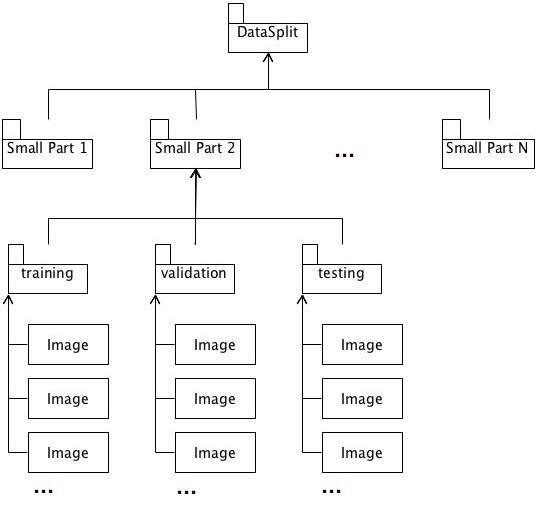
\includegraphics[width=\textwidth]{FS}
\caption{Dataset File Structure}
\label{fig:FS}
\end{figure}
%\section{Global Software Control}

%\textit{Note: Optional section describing describing the control flow of the system, in particular, whether a monolithic, event-driven control flow or concurrent processes have been selected, how requests are initiated and specific synchronization issues}


%\section{Boundary Conditions}

%\textit{Note: Optional section describing the use cases how to start up the separate components of the system, how to shut them down, and what to do if a component or the system fails.}










%------- CHAPTER 6 -------

\chapter{Case Study / Evaluation}

\textit{Note: If you did an evaluation / case study, describe it here.}

\section{Design}

\textit{Note: Describe the design / methodology of the evaluation and why you did it like that. E.g. what kind of evaluation have you done (e.g. questionnaire, personal interviews, simulation, quantitative analysis of metrics, what kind of participants, what kind of questions, what was the procedure?}

\section{Objectives}

\textit{Note: Derive concrete objectives / hypotheses for this evaluation from the general ones in the introduction.}

\section{Results}

\textit{Note: Summarize the most interesting results of your evaluation (without interpretation). Additional results can be put into the appendix.}

\section{Findings}

\textit{Note: Interpret the results and conclude interesting findings}

\section{Discussion}

\textit{Note: Discuss the findings in more detail and also review possible disadvantages that you found}

\section{Limitations}

\textit{Note: Describe limitations and threats to validity of your evaluation, e.g. reliability, generalizability, selection bias, researcher bias}











%------- CHAPTER 7 -------

\chapter{Summary}

\textit{Note: This chapter includes the status of your thesis, a conclusion and an outlook about future work.}

\section{Status}

\textit{Note: Describe honestly the achieved goals (e.g. the well implemented and tested use cases) and the open goals here. if you only have achieved goals, you did something wrong in your analysis.}

\subsection{Realized Goals}

\textit{Note: Summarize the achieved goals by repeating the realized requirements or use cases stating how you realized them.}

\subsection{Open Goals}

\textit{Note: Summarize the open goals by repeating the open requirements or use cases and explaining why you were not able to achieve them. \textbf{Important:} It might be suspicious, if you do not have open goals. This usually indicates that you did not thoroughly analyze your problems.}

\section{Conclusion}

\textit{Note: Recap shortly which problem you solved in your thesis and discuss your \textbf{contributions} here.}

\section{Future Work}

\textit{Note: Tell us the next steps  (that you would do if you have more time. be creative, visionary and open-minded here.}



\appendix

\chapter{Acronyms}

\begin{acronym}
\acro{SMP}{Small Mechanical Part}
\acro{DNN}{Deep Neural Network}
\acro{CNN}{Convolutional Neural Network}
\acro{SGD}{Stochastic Gradient Descent}
\acro{GPU}{Graphical Processing Unit}

\end{acronym}


\clearpage

\listoffigures
\clearpage

\listoftables
\clearpage

\bibliography{thesis}
\bibliographystyle{alpha}

\end{document}
